\chapter{Case Study on a Manufacturing Company}
\label{chap:casestudy}

In this chapter, the first three sections provide the implementation details along with the reason for making certain decisions regarding the implementation of web-based modeling tool. The fourth section provides an architecture of the functioning system and the fifth section provides application flow of the functioning system. The sixth section explains how motivating scenario has been modeled using the proposed modeling approach. Successful modeling of the motivating scenario using the developed editor serves as a proof for usability of the web-based modeling tool. Hence, the final section validates the system by evaluating it with the requirements for supporting intention-oriented organizational modeling. 

%%%%%%%%%%%%%%%%%%%%%%%%%%%%%%%%%%%%%%%%%%%%%%%%%%%%%%%%%%%%%%%%%%%%%%%%%
\section{Technologies and Frameworks}
\label{subsec:specifications}
%%%%%%%%%%%%%%%%%%%%%%%%%%%%%%%%%%%%%%%%%%%%%%%%%%%%%%%%%%%%%%%%%%%%%%%%%
In order to, realize the approach presented in the Section \ref{sec:topdownapproach} of the previous Chapter \ref{chap:approach}, a formal inquiry was done to choose suitable technologies and frameworks required. The below specifications were finalized and \textit{single page web application} (SPA) using\textit{client-side scripting} was chosen. The single page web application is a web application that fits on a single web browser page with user experience similar to a desktop application. In a SPA, the necessary code is retrieved within a single page load and they are easily updated and distributed, usually without requiring any action from the user \cite{Mikowski2013}. The client side scripting refers to the script code that is executed on the user's web browser instead on the web server \cite{Sierra2012}. The reason for selecting client side scripting is because of their advantages such as (1) no refreshing of the page while using the application, (2) suitable for applications that uses Javascript framework for evaluating SPA, etc. 

\begin{enumerate}   
	\item \textit{ClojureScript}\footnote{http://clojure.org/about/clojurescript} as the programming language
	\item \textit{Model-view-controller (MVC)} \cite{Deacon2009}  as the architecture pattern
	\item \textit{Re-frame}\footnote{https://github.com/Day8/re-frame} as the pattern for writing SPA in ClojureScript, using Reagent\footnote{http://reagent-project.github.io/}	
\end{enumerate}

Other than the above listed frameworks and technologies, frameworks like \textit{react-bootstrap}\footnote{https://react-bootstrap.github.io/}, jquery\footnote{https://jquery.com/} were also used, to provide more optimal view of the tool. Along with this, we have also used libraries like bidi\footnote{https://github.com/juxt/bidi} and pushy\footnote{https://github.com/kibu-australia/pushy}, to handle page navigation from current location to the desired location in the URL (Uniform Resource Locator) of the browser. 

%%%%%%%%%%%%%%%%%%%%%%%%%%%%%%%%%%%%%%%%%%%%%%%%%%%%%%%%%%%%%%%%%%%%%%%%%
\subsection{MVC Architecture}
\label{subsec:mvcarch}
%%%%%%%%%%%%%%%%%%%%%%%%%%%%%%%%%%%%%%%%%%%%%%%%%%%%%%%%%%%%%%%%%%%%%%%%%
The architecture of the developed user interface is based on the MVC design pattern. The MVC paradigm allows to separate business logic from the code that controls presentation of user interface and event handling \cite{Oracle2016}. Each entity view in the web page is made as a combination of at least one model, view and one or more controls. 

\textit{Model} stores the required data structure for web-based modeling tool. In the developed model, the data structure of modeling elements with their values are stored. 

\textit{View} contains HTML (HyperText Markup Language) elements and HTML constructs that describe the way of displaying the data from Model to the user. Most of the common functionalities that render user interface components are re-used. 

\textit{Control} contains the handler functions which can only change the model. Even the initial values of the model are put inside the control. This has functions that updates default database, which then re-renders the view. 

Apart from the above, there is another important component that registers subscription functions, i.e., query layer of the data. Subscription functions returns values that change over time, i.e., based on user events.

%%%%%%%%%%%%%%%%%%%%%%%%%%%%%%%%%%%%%%%%%%%%%%%%%%%%%%%%%%%%%%%%%%%%%%%%%
\subsubsection{Example: Component using the MVC Pattern }
%%%%%%%%%%%%%%%%%%%%%%%%%%%%%%%%%%%%%%%%%%%%%%%%%%%%%%%%%%%%%%%%%%%%%%%%%
The Figure \ref{fig:mvc_pattern} below shows how components interact with each other using the MVC pattern with a simple example of adding new modeling element. This functionality is same for all the types such as intentions, strategies, capabilities and informal processes.  

\begin{figure}
	\centering
	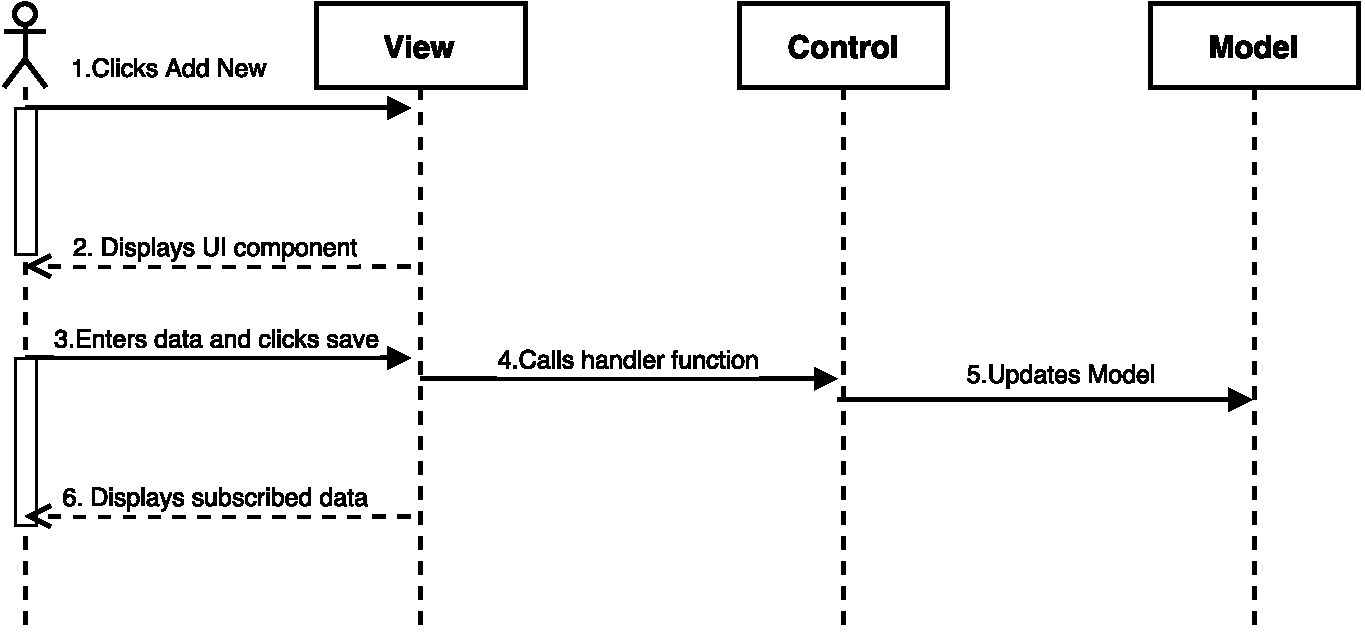
\includegraphics [width= \textwidth]{mvc_pattern.pdf}
	\caption{MVC Pattern of Adding New Modeling Element}
	\label{fig:mvc_pattern}
\end{figure}

\begin{enumerate}
	\item User clicks the \textit{Add New} button in the developed editor.
	\item Responding to the user click, view displays the respective user interface component for entering the new modeling element details.
	\item User enters the required basic details for adding new element and clicks save button.
	\item View dispatches data to control, as control can only modify the model.
	\item Control inserts/updates data into the model.
	\item View displays the updated model as it has been subscribed to the model.
\end{enumerate}

%%%%%%%%%%%%%%%%%%%%%%%%%%%%%%%%%%%%%%%%%%%%%%%%%%%%%%%%%%%%%%%%%%%%%%%%%
\section{Architecture of the Functioning System}
\label{sec:architectureofthefunctioningsystem}
%%%%%%%%%%%%%%%%%%%%%%%%%%%%%%%%%%%%%%%%%%%%%%%%%%%%%%%%%%%%%%%%%%%%%%%%%
Also from the Figure \ref{fig:architectureofthecasestudy}, it is clear that we followed the MVC architecture to design the user interface. Business experts can use the web-based modeling tool to view and update the descriptive information of the modeling elements. Whenever a change in the model data is detected respective handler function is \textit{dispatched} and the corresponding handler function can only \textit{update} the model. Since we associate every modeling element with another modeling element, model data of an element is required by another element which are resolved using the unique reference identifier. For example, intention model's unique reference identifier of intention \textit{improve help customer help portal} is required by the strategy \textit{through application development}. This is because, for strategy (through application development), intention (improve help customer help portal) is the target intention. 

\begin{figure}
	\centering
	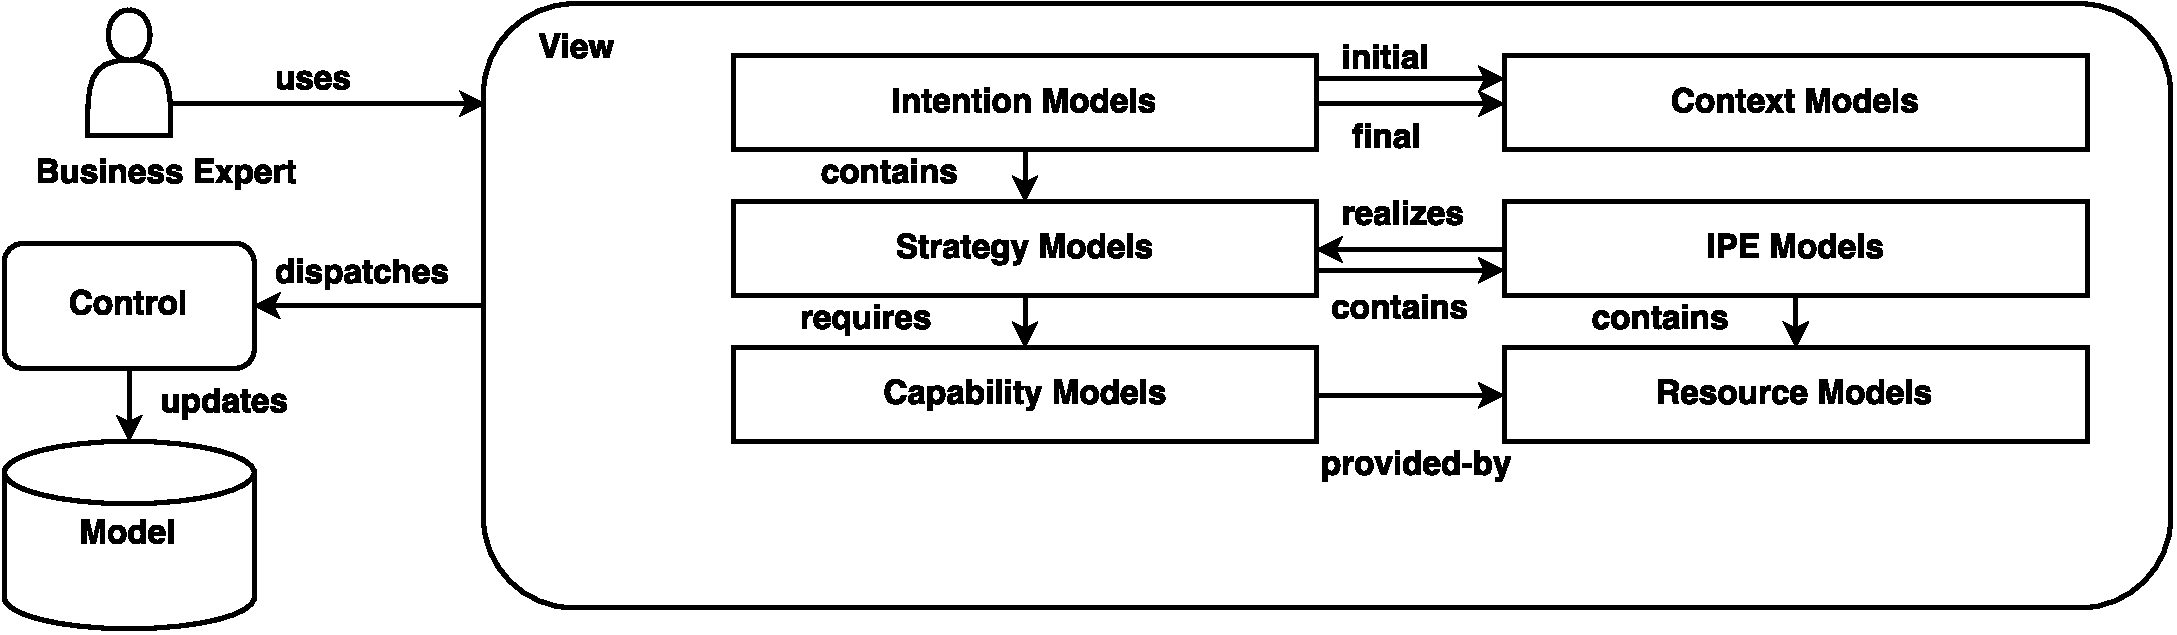
\includegraphics [width= \textwidth]{architectureofthecasestudy.pdf}
	\caption{Architecture of the Functioning System}
	\label{fig:architectureofthecasestudy}
\end{figure}


%%%%%%%%%%%%%%%%%%%%%%%%%%%%%%%%%%%%%%%%%%%%%%%%%%%%%%%%%%%%%%%%%%%%%%%%%
\subsection{Application Flow}
\label{subsec:applicationflow}
%%%%%%%%%%%%%%%%%%%%%%%%%%%%%%%%%%%%%%%%%%%%%%%%%%%%%%%%%%%%%%%%%%%%%%%%%
 In this subsection, we provide an overview about how page navigation from current location to the desired location happens in URL of the browser. The external libraries used for route navigation, parses the URL into data structures and generates URL from the data structure defined as required routes. We call a function to dispatch the route, with the matched route. Then we also have another function that parses the URL, to turn the URL into data structure representing it. From the Figure \ref{fig:UIArchitecture}, it is clear that route navigation for each entity items happens based on their entity type, e.g., intentions, strategies, etc., and its own unique reference identifier.

\begin{figure}
	\centering
	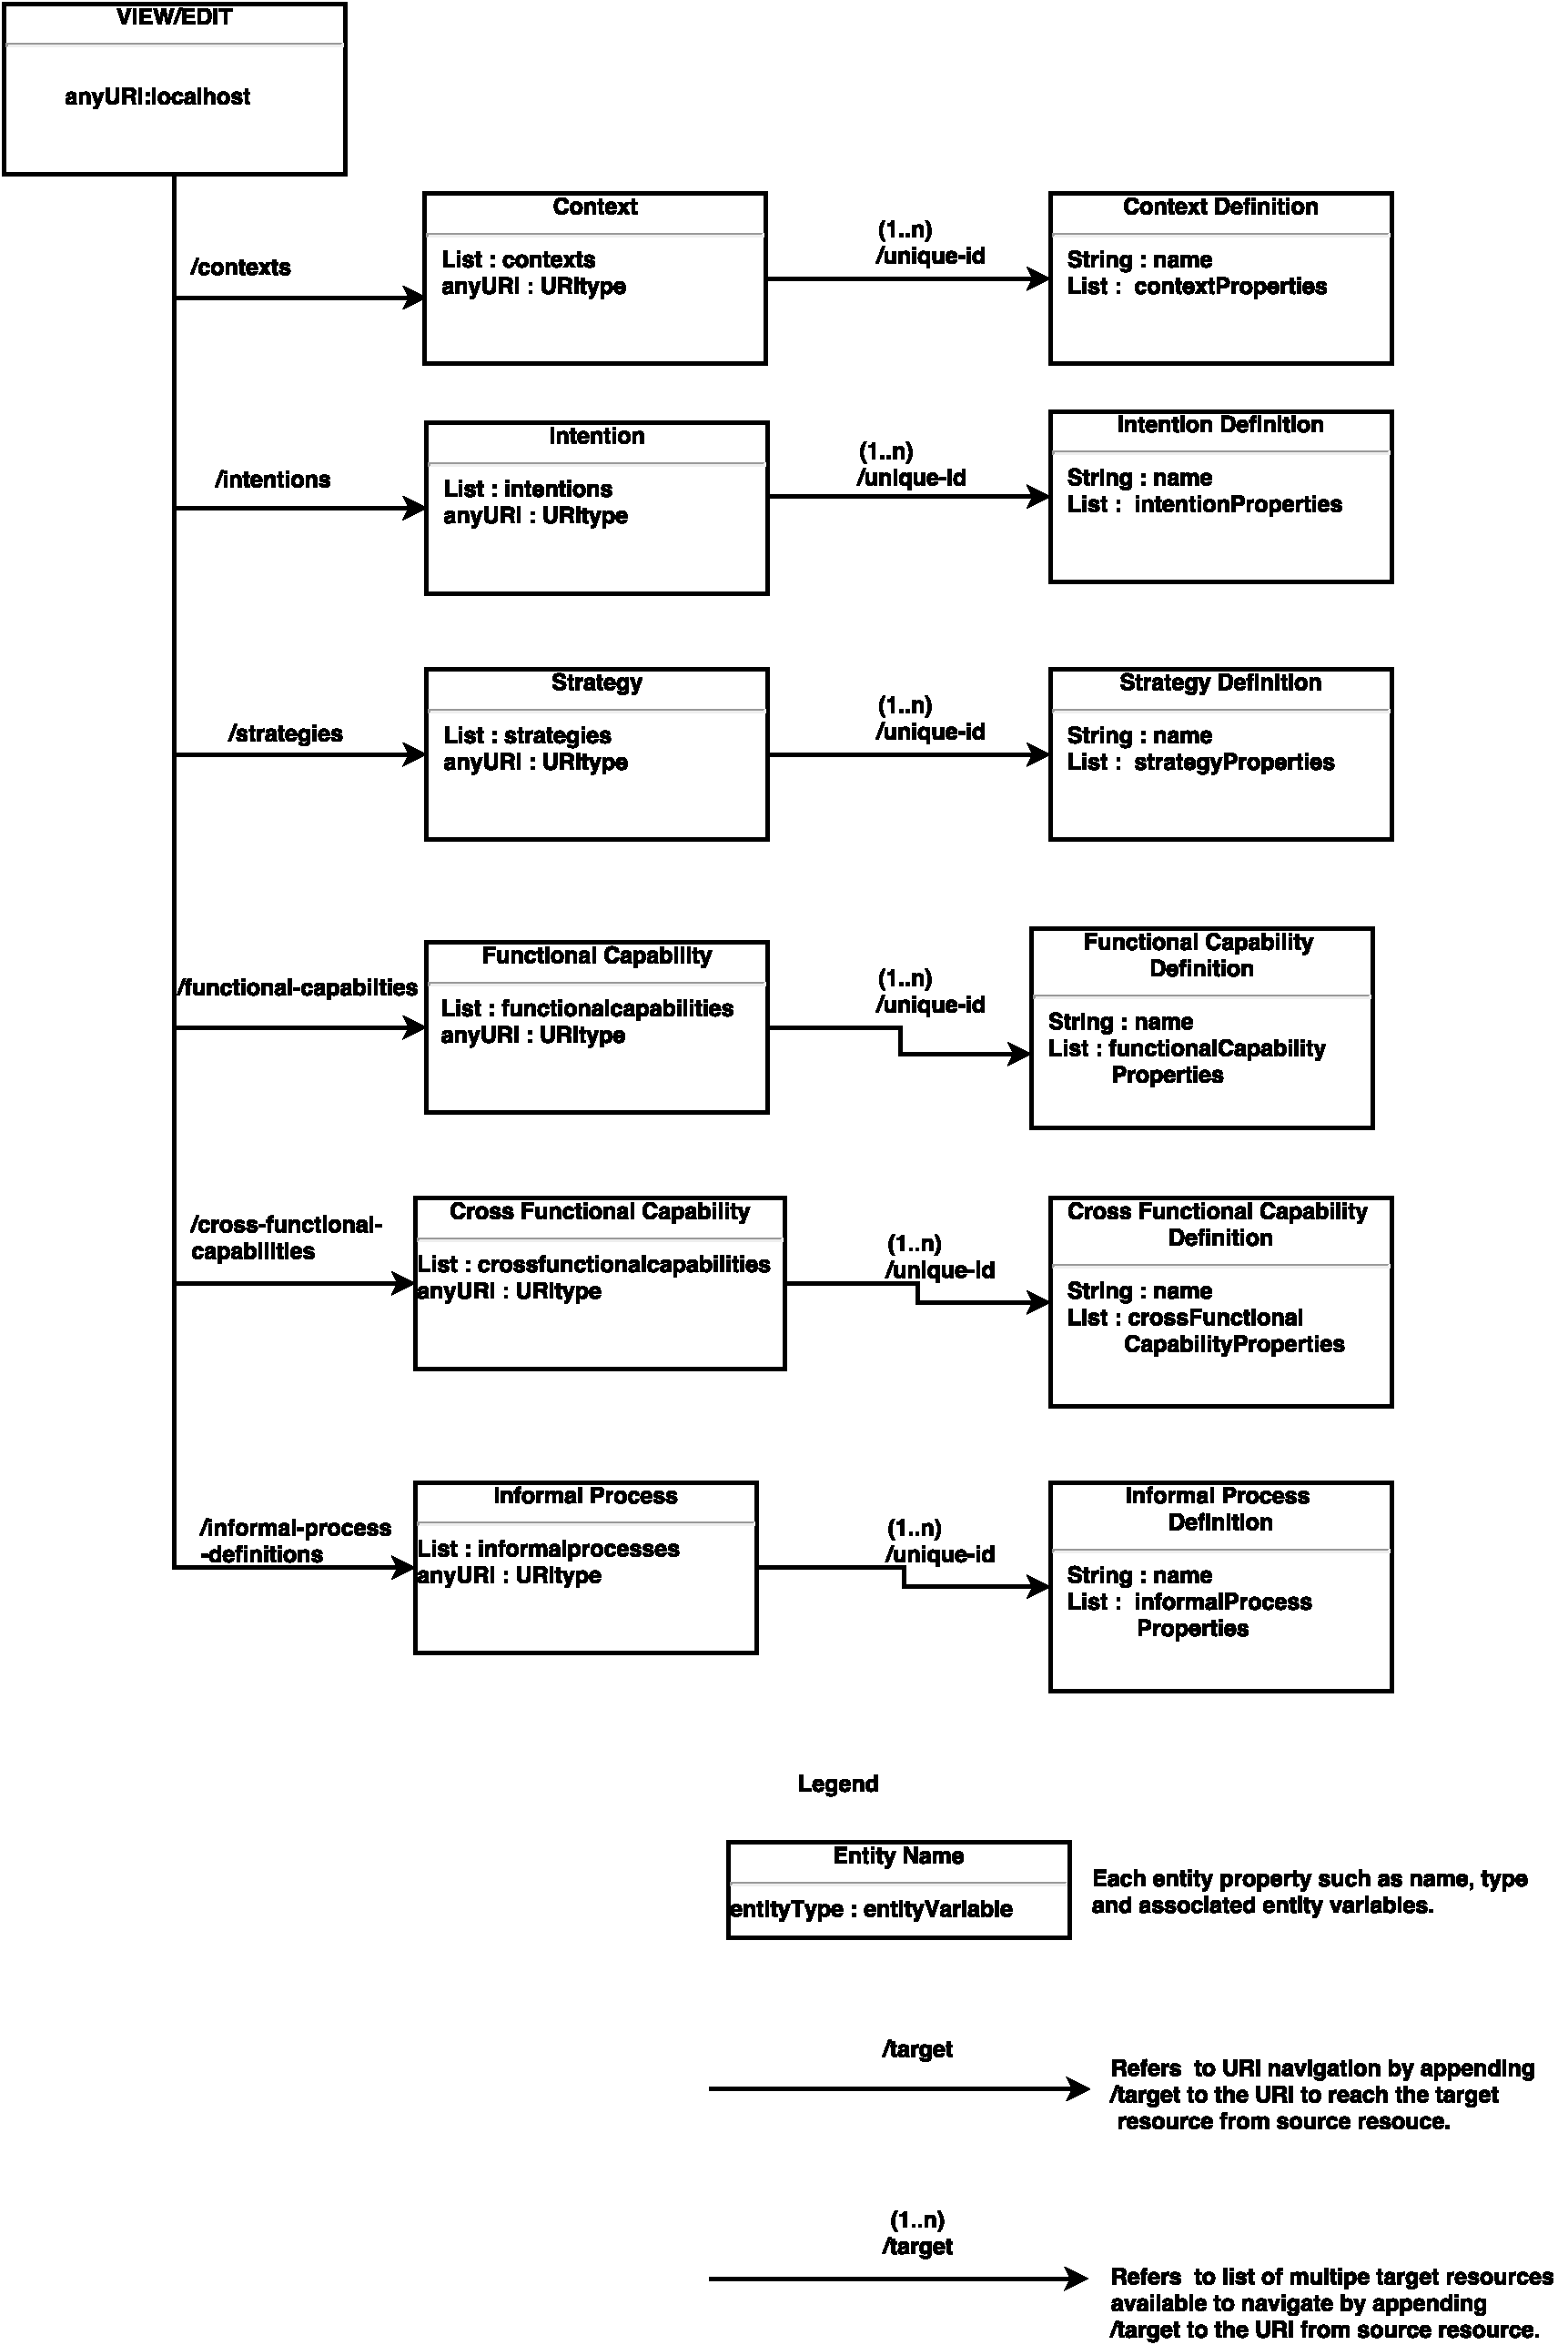
\includegraphics [width= \textwidth]{UIArchitecture.pdf}
	\caption{Implementation of the URL Navigation}
	\label{fig:UIArchitecture}
\end{figure} 

Each entity item has basic properties such as \textit{name} and \textit{target namespace}. The entities are identified using their unique id which is generated using the unique combination of name and target namespace. The entities that are associated with a particular entity are resolved through unique identifier. For example, in our motivating scenario consider the intention \textit{improve the customer help desk portal} when creating model for this intention, business expert provide name and namespace for this intention and add it to the database. A unique identifier is generated for the intention model using the combination of name and namespace by the system. For example, the strategy in the motivating scenario \textit{through application  development} that is associated with an intention, contains only the unique identifier of intention as reference. 

%%%%%%%%%%%%%%%%%%%%%%%%%%%%%%%%%%%%%%%%%%%%%%%%%%%%%%%%%%%%%%%%%%%%%%%%%
\section{User Interface Design of the Modeling Tool}
\label{sec:designmethodology}
%%%%%%%%%%%%%%%%%%%%%%%%%%%%%%%%%%%%%%%%%%%%%%%%%%%%%%%%%%%%%%%%%%%%%%%%%
This section discusses in detail the methods followed for designing the web-based modeling tool. The developed tool realizes the approach proposed in the Section \ref{sec:topdownapproach}. When designing the user interface components and functionalities, most of the similar functionalities are designed as common functions for the purpose of reusing the functions. This reduced unnecessary functional redundancies and overhead. It is also important to provide an introduction about the user interface design of the modeling tool, as it helps in understanding the following sections. Also to ensure consistency of the design, all the modeling elements' layout have similar user interface design as follows:



\subsection{Basic Properties}
From the Figure \ref{fig:samplescreen}, we could see that basic properties such as name and target namespace of a modeling element are displayed under the basic properties tab. For informal process models alone, we have another basic property that has the process type value of the process. 

\begin{figure}[H]
	\centering
	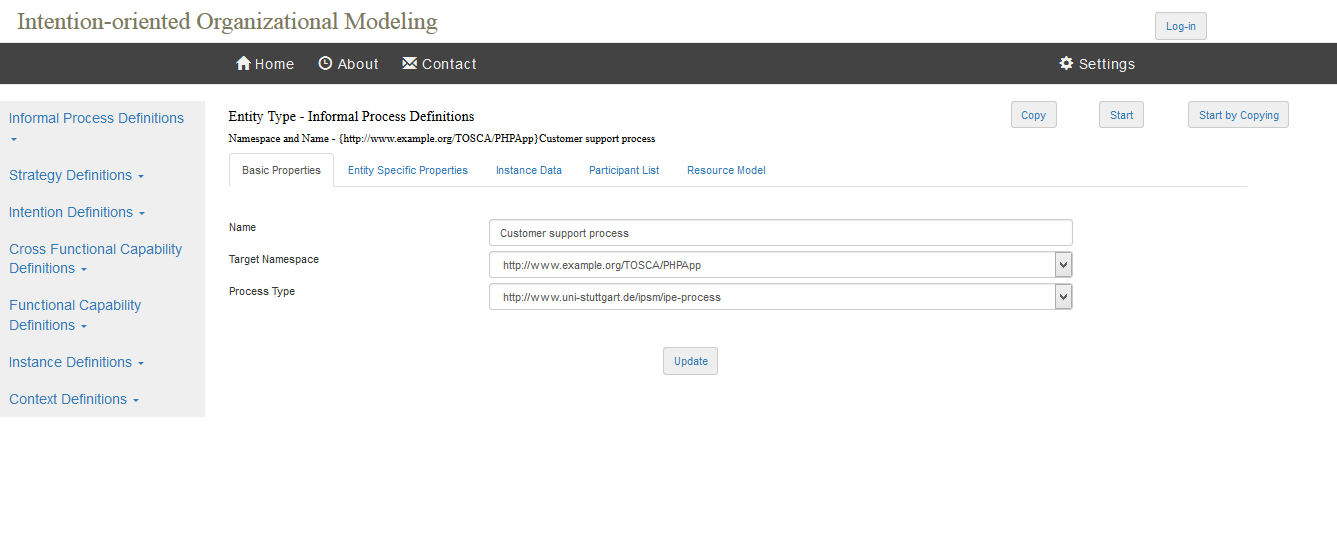
\includegraphics[width=\textwidth,angle=0]{Design_UI.png}
	\caption{User Interface Design of the Basic Properties Tab}
	\label{fig:samplescreen}
\end{figure}

\subsection{Entity Specific Properties}
The entity specific properties of a modeling element are displayed under this tab. The entity specific properties differ for each entity type, i.e., intention, strategy, etc. For example, intention models contain achieving strategies, related intentions, etc., under entity specific properties tab but strategy models contain details like target intentions, required organizational capabilities, etc. From the Figure \ref{fig:samplescreen_esp}, we could see that entity specific properties of a process model includes details of associated contexts, intentions and estimated cost of the process model.

\begin{figure} [H]
	\centering
	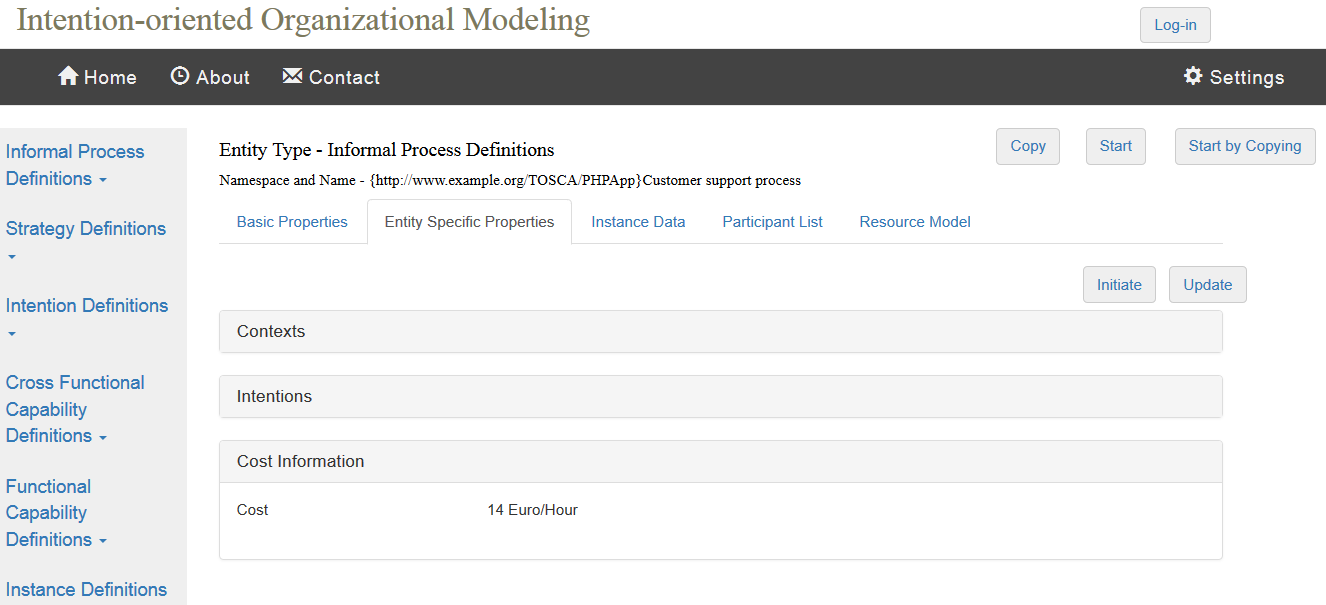
\includegraphics[width=\textwidth,angle=0]{Design_UI_ESP.png}
	\caption{User Interface Design of the Entity Specific Properties Tab}
	\label{fig:samplescreen_esp}
\end{figure}

\subsection{Participant List}
Since intention-oriented organizational modeling satisfies the requirement of participative organizational modeling, we provide participant list tab. This tab holds details of organizational members and their respective privileges. The current design includes only adding and removing of the organizational members as participants. The design also includes assigning privileges to participants such as priviliege to edit, view, follow and own. But the current functioning system, could not check if the members do work based on their privileges. For example, consider a participant who has privilege to only view an intention model and suppose if the participant edits the model then the functioning system does not have functionalities to prevent him from doing so. From the Figure \ref{fig:samplescreen_pl}, we could see that participant list tab of a modeling element contains the details of participants those who can edit, view, follow or own a particular model. Also from the Figure \ref{fig:samplescreen_pl_editor}, we could see how privileges for a particular participant can be provided and revoked by adding or removing a participant under particular privilege.  
\begin{figure} [H]
	\centering
	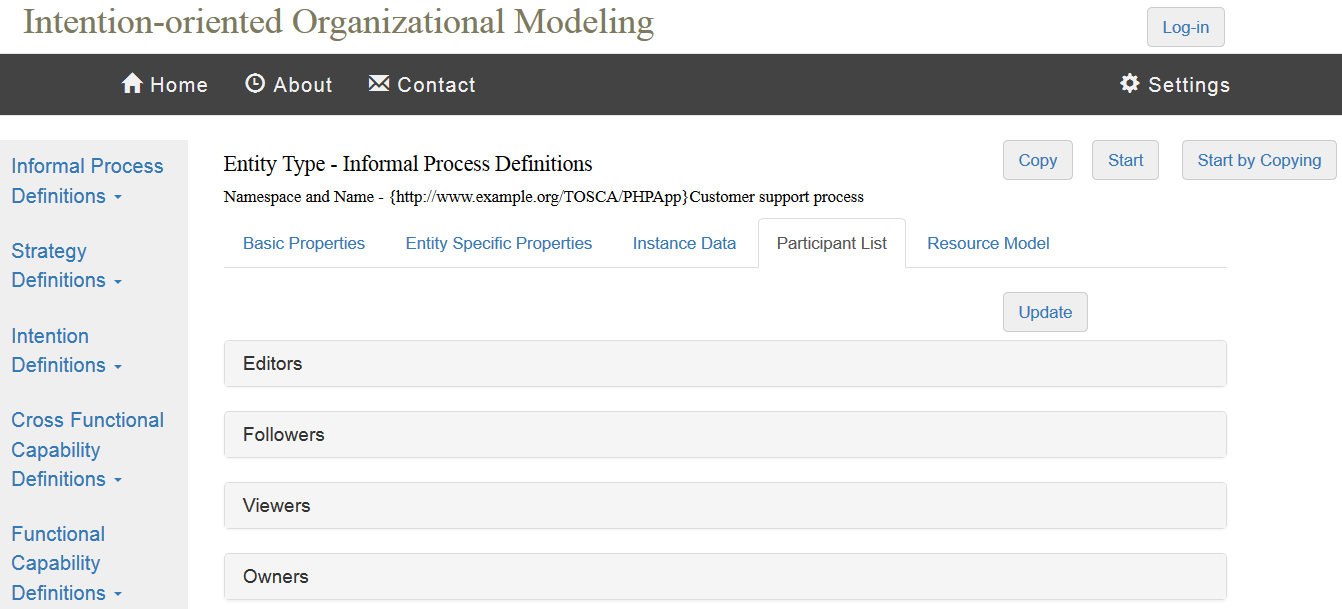
\includegraphics[width=\textwidth,angle=0]{Design_UI_Participant_2.png}
	\caption{User Interface Design of the Participant List Tab}
	\label{fig:samplescreen_pl}
\end{figure}

\begin{figure} [H]
	\centering
	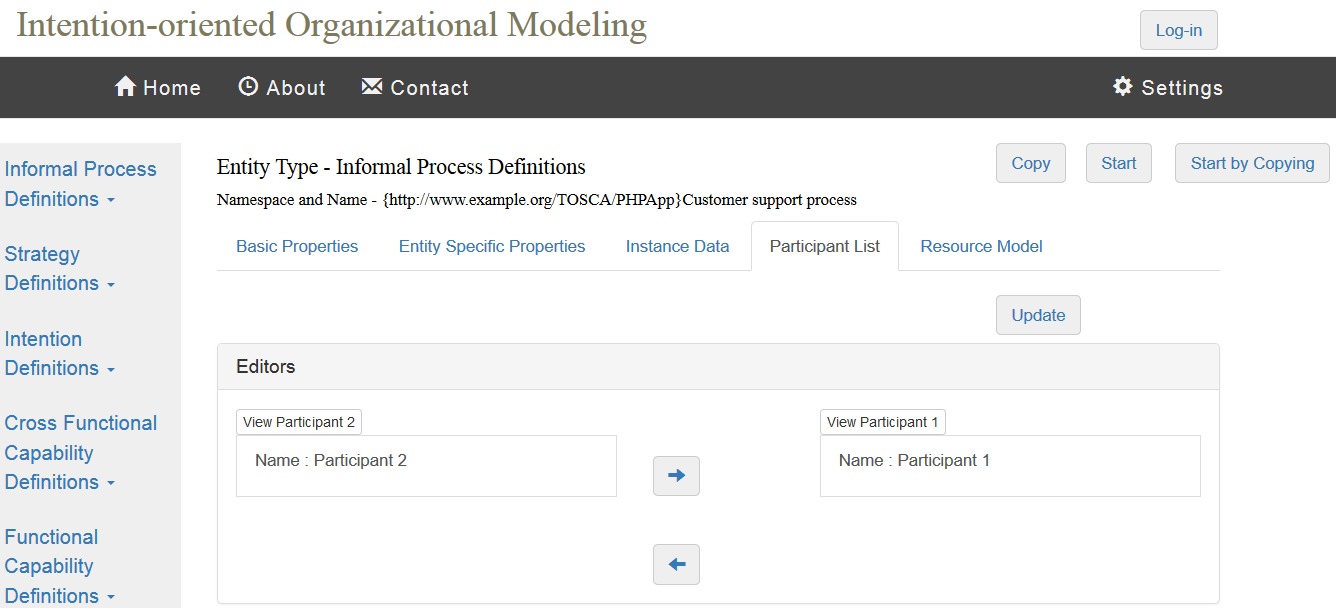
\includegraphics[width=\textwidth,angle=0]{Design_UI_Participant.png}
	\caption{User Interface Design of the Participant as an Editor of the Model}
	\label{fig:samplescreen_pl_editor}
\end{figure}

\subsection{Instance Data}
When a model is initialized, it results in a model instance. The instances contained under a model are shown inside the instance data tab. For example, the Figure \ref{fig:samplescreen_instance} shows the instance contained under an informal process model. 
  

\begin{figure} [H]
	\centering
	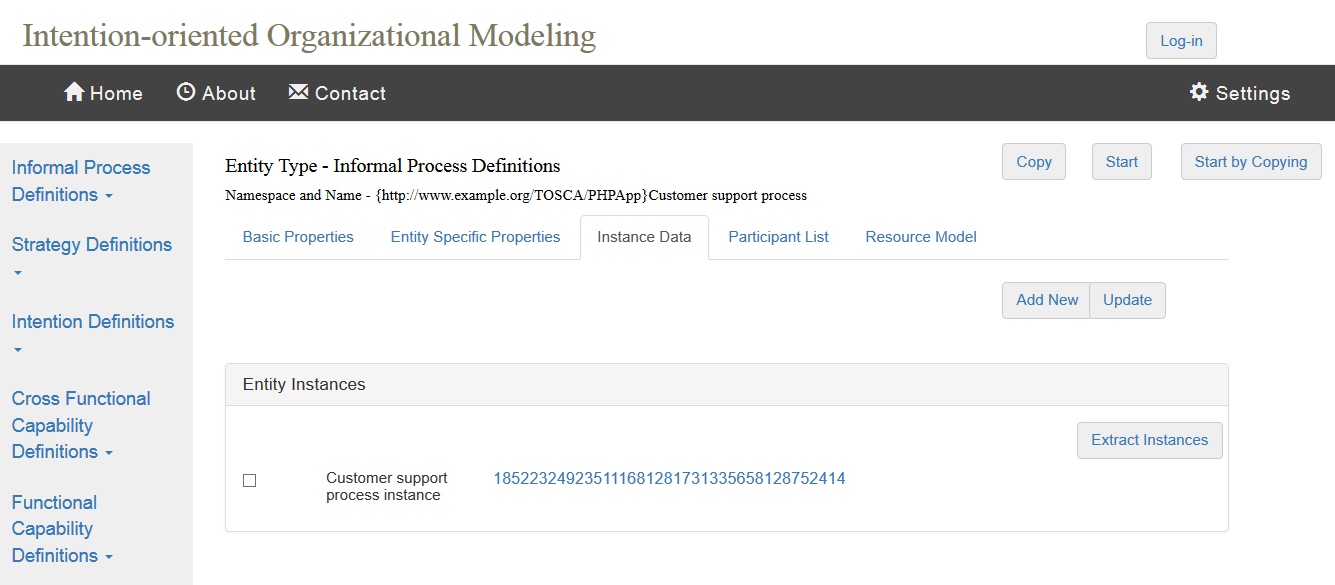
\includegraphics[width=\textwidth,angle=0]{Design_UI_InstanceData.png}
	\caption{User Interface Design of the Instance Data Tab}
	\label{fig:samplescreen_instance}
\end{figure}


Some of the important methodologies followed with respect to user interface components design are (1) multiple items to be selected from multiple list items are displayed as \textit{list group} and (2) selecting single item from multiple items are displayed as \textit{drop down}. For example, to select multiple strategies from a list of strategies, available strategies are displayed as a list from which the user can select desired number of strategies. Another important methodology followed during user interface design is, for every entity the properties should be displayed only under the respective properties tab. For example, in the Figure \ref{fig:samplescreen}, the basic properties such as name, target namespace and process type of an informal process model should be displayed only under the respective basic properties tab and similarly for all other tabs. This methodology is followed uniformly throughout the design of all the entity types such as intention definitions, strategy definitions, capability definitions, context definitions, instance definitions and informal process definitions. 

All data are stored only under the model. This applies to the labels and text fields of all user interface elements and this data can be updated only through the handler function. Through the \textit{settings} option, user can add new target namespace type and intention relation type. From the Figure \ref{fig:samplescreen}, it is clear that a consistent design methodology has been followed to display the list of available entity types such as intentions, strategies, capabilities etc., and to display their respective properties such as basic, entity specific, instance data, etc. Though the top-down modeling approach \ref{sec:topdownapproach}, shows that definition of each entity type is contained within another entity type, as per the user interface design, separate entities references each other using the unique reference identifier but does not contain all properties of referenced entity. For instance, a strategy containing an intention should contain only the intention's unique reference identifier but not the actual intention itself. Later in the view of strategy, actual intention properties are fetched and displayed based on the unique reference identifier. 


%%%%%%%%%%%%%%%%%%%%%%%%%%%%%%%%%%%%%%%%%%%%%%%%%%%%%%%%%%%%%%%%%%%%%%%%%
\section{Realization of the Approach}
\label{sec:realization}
%%%%%%%%%%%%%%%%%%%%%%%%%%%%%%%%%%%%%%%%%%%%%%%%%%%%%%%%%%%%%%%%%%%%%%%%%
In order to realize the proposed approach in the Section \ref{sec:topdownapproach} of Chapter \ref{chap:approach}, we create models using the developed web-based modeling tool for the motivating scenario discussed in the Chapter \ref{chap:motivatingScenario}. It is also important to model them step by step as mentioned in the Section \ref{sec:informalprocessmodeling}. As we mentioned earlier, to realize the approach in organizations, we model the motivating scenario step by step as mentioned in the second phase of the InProXec method. As each models are designed in an individual modeling step, details of individual modeling steps are provided in the following subsections. This section helps to understand the usability of the approach in the organizations. The user interface screen design of the below modeling elements are consistent and similar to the screen design explained in the previous Section \ref{sec:designmethodology}.

%%%%%%%%%%%%%%%%%%%%%%%%%%%%%%%%%%%%%%%%%%%%%%%%%%%%%%%%%%%%%%%%%%%%%%%%%
\subsection{Modeling of the Contexts}
%%%%%%%%%%%%%%%%%%%%%%%%%%%%%%%%%%%%%%%%%%%%%%%%%%%%%%%%%%%%%%%%%%%%%%%%%
In the informal process modeling approach, the first modeling step is to model the context definitions (M1). Each informal process starts from an initial context and aims to achieve an intention \cite{Sungur2014a}. After reaching an intention, there is resulting IPE Context. To model the contexts, user can add new contexts by providing basic properties such as name of the context and target namespace of the context as they serve as unique reference identifier for these contexts. After successfully adding the basic properties, user can provide entity specific properties such as contained contexts inside the main context, entity definition details about the contexts and participant list with respective privileges for each participant are also provided. The required context definitions are modeled first because these definition are required for modeling intention definitions and process definitions. For example, to model the contexts in our motivating scenario we can provide details of the initial context and final context. 

%%%%%%%%%%%%%%%%%%%%%%%%%%%%%%%%%%%%%%%%%%%%%%%%%%%%%%%%%%%%%%%%%%%%%%%%%
\subsection{Modeling of the Intentions}
%%%%%%%%%%%%%%%%%%%%%%%%%%%%%%%%%%%%%%%%%%%%%%%%%%%%%%%%%%%%%%%%%%%%%%%%%
After modeling context definitions(M1), the second step of the modeling is to model the intentions (M2). For example, in our motivating scenario we have main intention as "increase revenue and number of unit sales" and other low level intentions that emerged out of main intention and strategies of the main intention. The user can provide descriptive information about particular intention as intention definition. Similar to context modeling, the user has to provide basic properties such as name and target namespace required for unique identification of the entity. After providing basic properties, the user has to provide entity specific details of the intention such as due date and time for intention completion, priority of the intention, cost of the intention, other related intentions that are contained under this particular intention. The strategies to achieve this intention and contexts of the intention are also provided as entity specific properties. The participant list with respective privileges for each participant are also provided when an entity is of type interactive acquirable entity. 

%%%%%%%%%%%%%%%%%%%%%%%%%%%%%%%%%%%%%%%%%%%%%%%%%%%%%%%%%%%%%%%%%%%%%%%%%
\subsection{Modeling of the Strategies}
%%%%%%%%%%%%%%%%%%%%%%%%%%%%%%%%%%%%%%%%%%%%%%%%%%%%%%%%%%%%%%%%%%%%%%%%%
After modeling context definitions (M1) and intention definitions (M2) user can proceed to model the strategies (M3) which is third step of the modeling process. For example, in our motivating scenario user can model the strategies such as \textit{through expansion}, \textit{through advertisements} and other required strategies as third step of the modeling process. Similar to earlier modeling steps, during modeling of strategy user required to provide basic properties such as name and target namespace. After providing the basic properties, entity specific properties such as target intentions of the strategy, capabilities and process definitions associated with strategy are also provided. Since, strategy is also an interactive acquirable entity similar to intention, participant list details are also provided during modeling of strategies

%%%%%%%%%%%%%%%%%%%%%%%%%%%%%%%%%%%%%%%%%%%%%%%%%%%%%%%%%%%%%%%%%%%%%%%%%
\subsection{Modeling of the Capabilities}
%%%%%%%%%%%%%%%%%%%%%%%%%%%%%%%%%%%%%%%%%%%%%%%%%%%%%%%%%%%%%%%%%%%%%%%%%
Modeling of capability (M4) is the fourth step in intention-oriented organizational modeling. There are two types of capabilities. Functional capabilities and cross-functional capabilities. Functional capabilities are the capabilites that associated with other entity types. Cross-functional capabilities contains multiple functional capabilities. Similar to earlier entity types' basic properties such as name and target namespace are added to get the unique reference identifier and entity specific properties for capabilities are added. Since cross functional capability contains functional capabilities, it holds the identifiers of the functional capabilities contained in it. Functional capability definitions also has participant list details similar to intention definitions and strategy definitions. 

%%%%%%%%%%%%%%%%%%%%%%%%%%%%%%%%%%%%%%%%%%%%%%%%%%%%%%%%%%%%%%%%%%%%%%%%%
\subsection{Modeling of the Resources}
%%%%%%%%%%%%%%%%%%%%%%%%%%%%%%%%%%%%%%%%%%%%%%%%%%%%%%%%%%%%%%%%%%%%%%%%%
Each resource that provides certain capability can be related to another resource which are defined using predefined or custom \textit{relationships} \cite{Sungur2014a}. In the developed modeling tool, the resource models are managed by embedding the open source modeling tool Winery \cite{Kopp2013} in the modeling tool's resource model tab. This is because Winery offers resources which we can model using their tool that is embedded under the resource model tab.

%%%%%%%%%%%%%%%%%%%%%%%%%%%%%%%%%%%%%%%%%%%%%%%%%%%%%%%%%%%%%%%%%%%%%%%%%
\subsection{Modeling of the Instances}
%%%%%%%%%%%%%%%%%%%%%%%%%%%%%%%%%%%%%%%%%%%%%%%%%%%%%%%%%%%%%%%%%%%%%%%%%		
 A model instance contains additional meta-data about the executed processes such as the information about the start date and time, end date and time, instance status, cost, source model etc. From the screen-shot image \ref{fig:realizationofinstances} it is clear that these properties of an instance can be edited through the developed tool. The developed tool supports creation and updation of descriptive information about instances. Each instance belong to any one of the acquirable entity type such strategies, intentions and informal processes. Any modeling element that has instances are also listed inside the \textit{Instance data} tab of each modeling element.  
 
\begin{figure} [H]
	\centering
	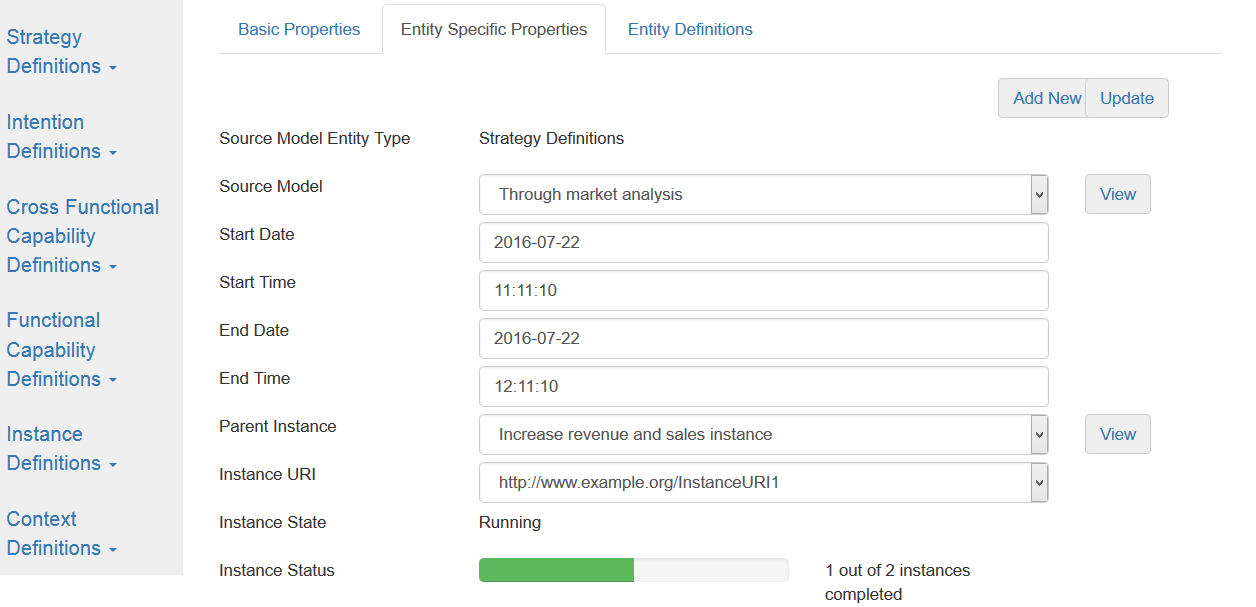
\includegraphics[width=\textwidth,angle=0]{Design_UI_Instance.png}
	\caption{User Interface Screen of an Instance Model}
	\label{fig:realizationofinstances}
\end{figure}

%%%%%%%%%%%%%%%%%%%%%%%%%%%%%%%%%%%%%%%%%%%%%%%%%%%%%%%%%%%%%%%%%%%%%%%%%
\section{Realization of the Requirements}
\label{sec:validation}
%%%%%%%%%%%%%%%%%%%%%%%%%%%%%%%%%%%%%%%%%%%%%%%%%%%%%%%%%%%%%%%%%%%%%%%%%	
This section provides details of realizing the requirements of intention-oriented organizational modeling that are satisfied by the proposed approach. Though we validated the approach using the requirements in the Section \ref{sec:topdownapproach} of the previous Chapter \ref{chap:approach}, it is important to mention the realization of the requirements by the tool.

\textit{Organizational Intention Transparency} (R1):  Using the modeling tool intentions at different levels can be modeled which satisfies first prerequisite of R1. With the current functioning system any user can view intention at different levels which satisfies second prerequisite of R2. Thus, the functioning tool realizes the requirement R1.

\textit{Organizational Strategy-based Cost Estimation} (R2): The cost of the organizational resources are stored. The modeling tool itself calculates and displays the estimated strategy cost calculation based on strategy implementation and resource cost. This cost information helps the business experts to make certain decision based on cost calculation during modeling. Thus, the functioning tool realizes the requirement R2.  

\textit{Organizational Strategy Achievability Estimation} (R3): Similar to cost calculation, strategy achievability estimation based on its association with valid capability is also determined and displayed during modeling phase itself. Thus, the functioning tool realizes the requirement R3.

\textit{Intention Oriented Working Style} (R4): Any user can create intention models, strategy models, informal process models etc., through the developed tool provided the user has understanding about main intention and its recursive structure. Thus, the functioning tool realizes the requirement R4.

\textit{Participative Organizational Modeling} (R5): With the current functioning system, any user can provide inputs for participative organizational modeling. Thus, the tool satisfies the requirement R5.
		

